\documentclass[12pt,a4paper,openright,twoside]{book}
\usepackage[utf8]{inputenc}
\usepackage{disi-thesis}
\usepackage{code-lstlistings}
\usepackage{notes}
\usepackage{shortcuts}
\usepackage{acronym}

\school{\unibo}
\programme{Corso di Laurea Magistrale in Ingegneria e Scienze Informatiche}
\title{Fancy Title}
\author{Cecilia Teodorani}
\date{\today}
\subject{Project Management}
\supervisor{Prof. Marco Antonio Boschetti}
\cosupervisor{Dott. CoSupervisor 1}
\morecosupervisor{Dott. CoSupervisor 2}
\session{IV}
\academicyear{2023-2024}

% Definition of acronyms
\acrodef{IoT}{Internet of Thing}
\acrodef{vm}[VM]{Virtual Machine}


\mainlinespacing{1.241} % line spacing in mainmatter, comment to default (1)

\begin{document}

\frontmatter\frontispiece

\begin{abstract}	
    %Very brief (e.g. 250-300 words)
    %Context, Problem/Objectives, Methods/Contribution, Results, Conclusions

Il presente lavoro nasce dall’esigenza di \textit{Peer Network} di ottimizzare la gestione
dei progetti aziendali. L’azienda opera nel settore della digitalizzazione e re-ingegnerizzazione
dei processi per i propri clienti, sviluppando applicazioni componibili anziché software interamente
personalizzati. Ogni entità di business coinvolta viene implementata come un'unità modulare,
denominata \acl{PBC}, che integra sia i propri dati che le azioni eseguibili su di essa. Oltre a
realizzare soluzioni per i clienti con questo approccio, \textit{Peer Network} sviluppa internamente
nuove \acl{PBC} e un’applicazione gestionale interna, \acl{PAM}, volta a migliorare l’efficienza
delle attività amministrative e organizzative.

L’analisi è iniziata esaminando nel dettaglio tutte le fasi del ciclo di vita di un progetto, dalle
attività gestionali e operative iniziali, fino all’installazione del sistema e alla fase di supporto.
Successivamente, partendo dai principi teorici del \acl{PMBOK}, dall’esperienza maturata in altri contesti
lavorativi e considerando la necessità di non poter stravolgere il metodo di lavoro aziendale, sono state
proposte soluzioni pratiche per rendere più efficiente la gestione dei progetti.

Una delle soluzioni concretamente implementate in \acl{PAM} durante questo lavoro riguarda l’automazione
dell’inserimento e dell’aggiornamento dei dati economici di ciascun progetto, inclusi costi, ricavi e
margini, sia pianificati che effettivi. In precedenza, questa gestione avveniva manualmente tramite
fogli elettronici, con un dispendio di tempo e un maggior rischio di errore. L’integrazione in \acl{PAM}
consente invece di ridurre i tempi di compilazione, centralizzare i dati in un’unica piattaforma e migliorare
l'affidabilità delle informazioni grazie all’automazione di alcuni inserimenti e calcoli.

\end{abstract}

\begin{dedication} % this is optional
Optional. Max a few lines.
\end{dedication}

%----------------------------------------------------------------------------------------
\tableofcontents   
\listoffigures     % (optional) comment if empty
\lstlistoflistings % (optional) comment if empty
%----------------------------------------------------------------------------------------

\mainmatter

\chapter{Introduction}
\label{chap:introduction}

Write your intro here.
\sidenote{Add sidenotes in this way. They are named after the author of the thesis}

You can use acronyms that your defined previously,
such as \ac{IoT}.
%
If you use acronyms twice,
they will be written in full only once
(indeed, you can mention the \ac{IoT} now without it being fully explained).
%
In some cases, you may need a plural form of the acronym.
%
For instance,
that you are discussing \acp{vm},
you may need both \ac{vm} and \acp{vm}.

\paragraph{Structure of the Thesis}

\note{At the end, describe the structure of the paper}


\chapter{Progetto}
\label{chap:project}

\textit{Peer Network} supporta le aziende nella revisione e reingegnerizzazione dei processi aziendali, adottando un
approccio basato su \textbf{processi componibili}, un esempio è presente in \Cref{fig:composable-process}. Questo approccio
supera i limiti dei sistemi monolitici tradizionali, introducendo moduli autonomi, riutilizzabili e facilmente
combinabili, che garantiscono flessibilità e adattabilità di fronte ai cambiamenti operativi.

\begin{figure}
    \centering
    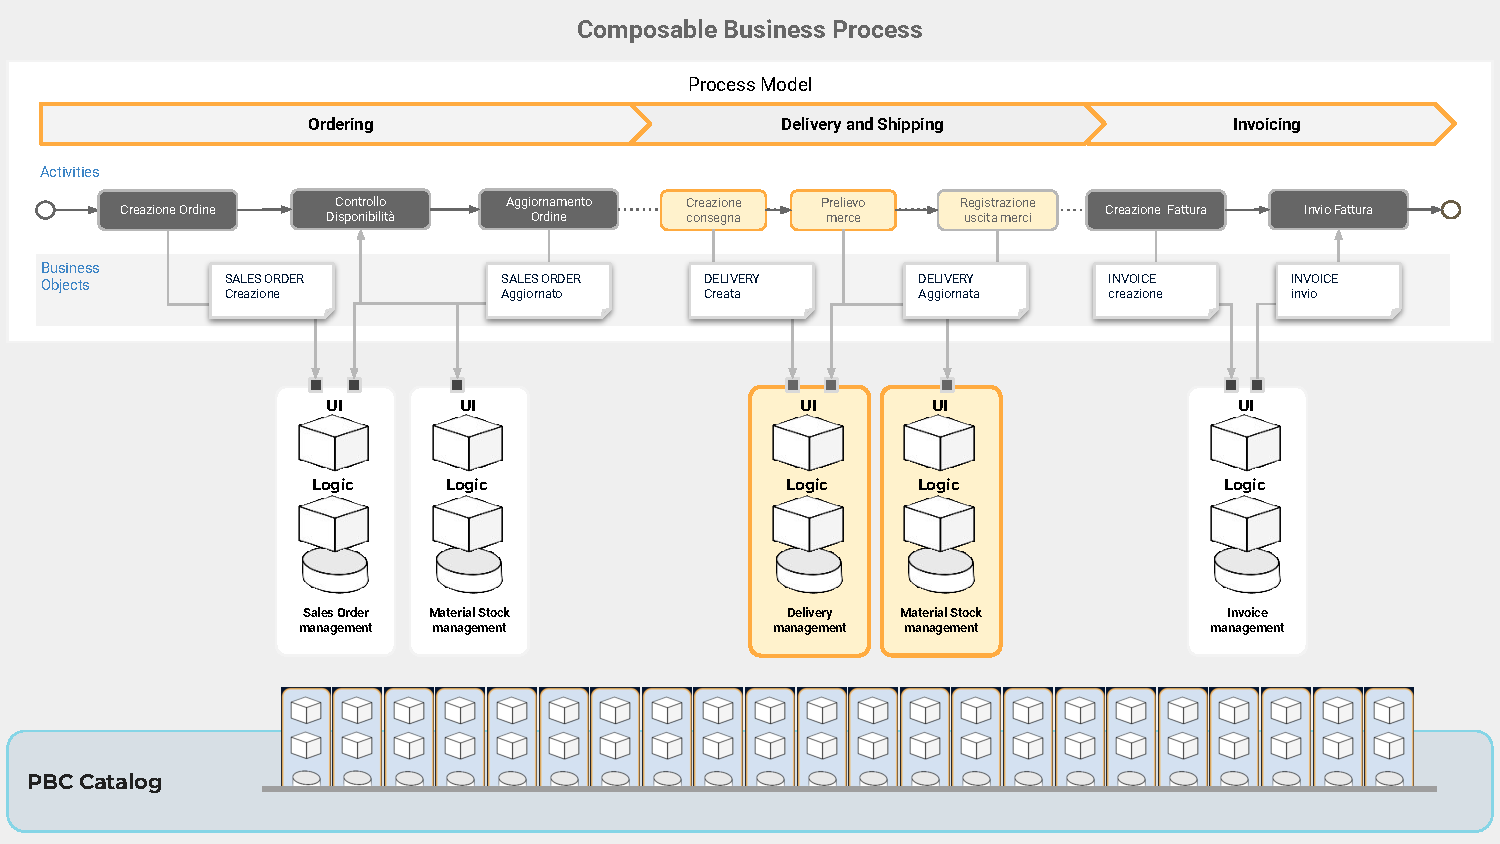
\includegraphics[width=\linewidth]{figures/composable_process.pdf}
    \caption{Struttura di un processo componibile}
    \label{fig:composable-process}
\end{figure}

La ridefinizione dei processi inizia identificando le attività da svolgere e gli \textbf{oggetti di business (BO)} coinvolti.
Gli oggetti di business rappresentano elementi chiave di un’organizzazione all’interno di un sistema informativo. Essi
riflettono entità reali, ad esempio cliente, prodotto, ordine, consegna, includendo ciascuno attributi specifici
(es. nell’ordine ci sono numero ordine, stato, riferimento ai prodotti). Questi oggetti, modellati in modo chiaro,
facilitano la gestione e l’integrazione dei processi aziendali, fungendo da base per la progettazione delle \ac{PBC}.

Per analizzare e modellare questi elementi, viene applicato il \textbf{Domain Driven Design}\cite{evans2004domain}, un metodo che consente di
suddividere il dominio aziendale in \textbf{Bounded Contexts} distinti. Ogni contesto rappresenta un sottoinsieme indipendente
e ben definito del dominio, facilitando la gestione e l’organizzazione dei processi.

All’interno di ciascun Bounded Context, gli oggetti di business vengono implementati come \textbf{\ac{PBC}}.
Queste unità modulari e riutilizzabili rappresentano specifiche entità aziendali che racchiudono in sé i dati e le azioni che
si possono compiere su di esse in un formato indipendente e facilmente integrabile. Come schematizzato nella \Cref{fig:pbc-struttura}
e nell’esempio in \Cref{fig:composable-process}, ciascuna \ac{PBC} descritta nelle ricerche di \textit{Gartner}\cite{natis2019innovation}\cite{burke2020top} include:

\begin{itemize}
    \item una \textbf{struttura dati} per rappresentare le informazioni associate alla \ac{PBC},
    \item un insieme di \textbf{API} di base per eseguire azioni sincrone sull'oggetto,
    \item un insieme di \textbf{eventi} di base per l'integrazione asincrona,
    \item una o più \textbf{interfacce utente} (opzionale).
\end{itemize}

\begin{figure}
    \centering
    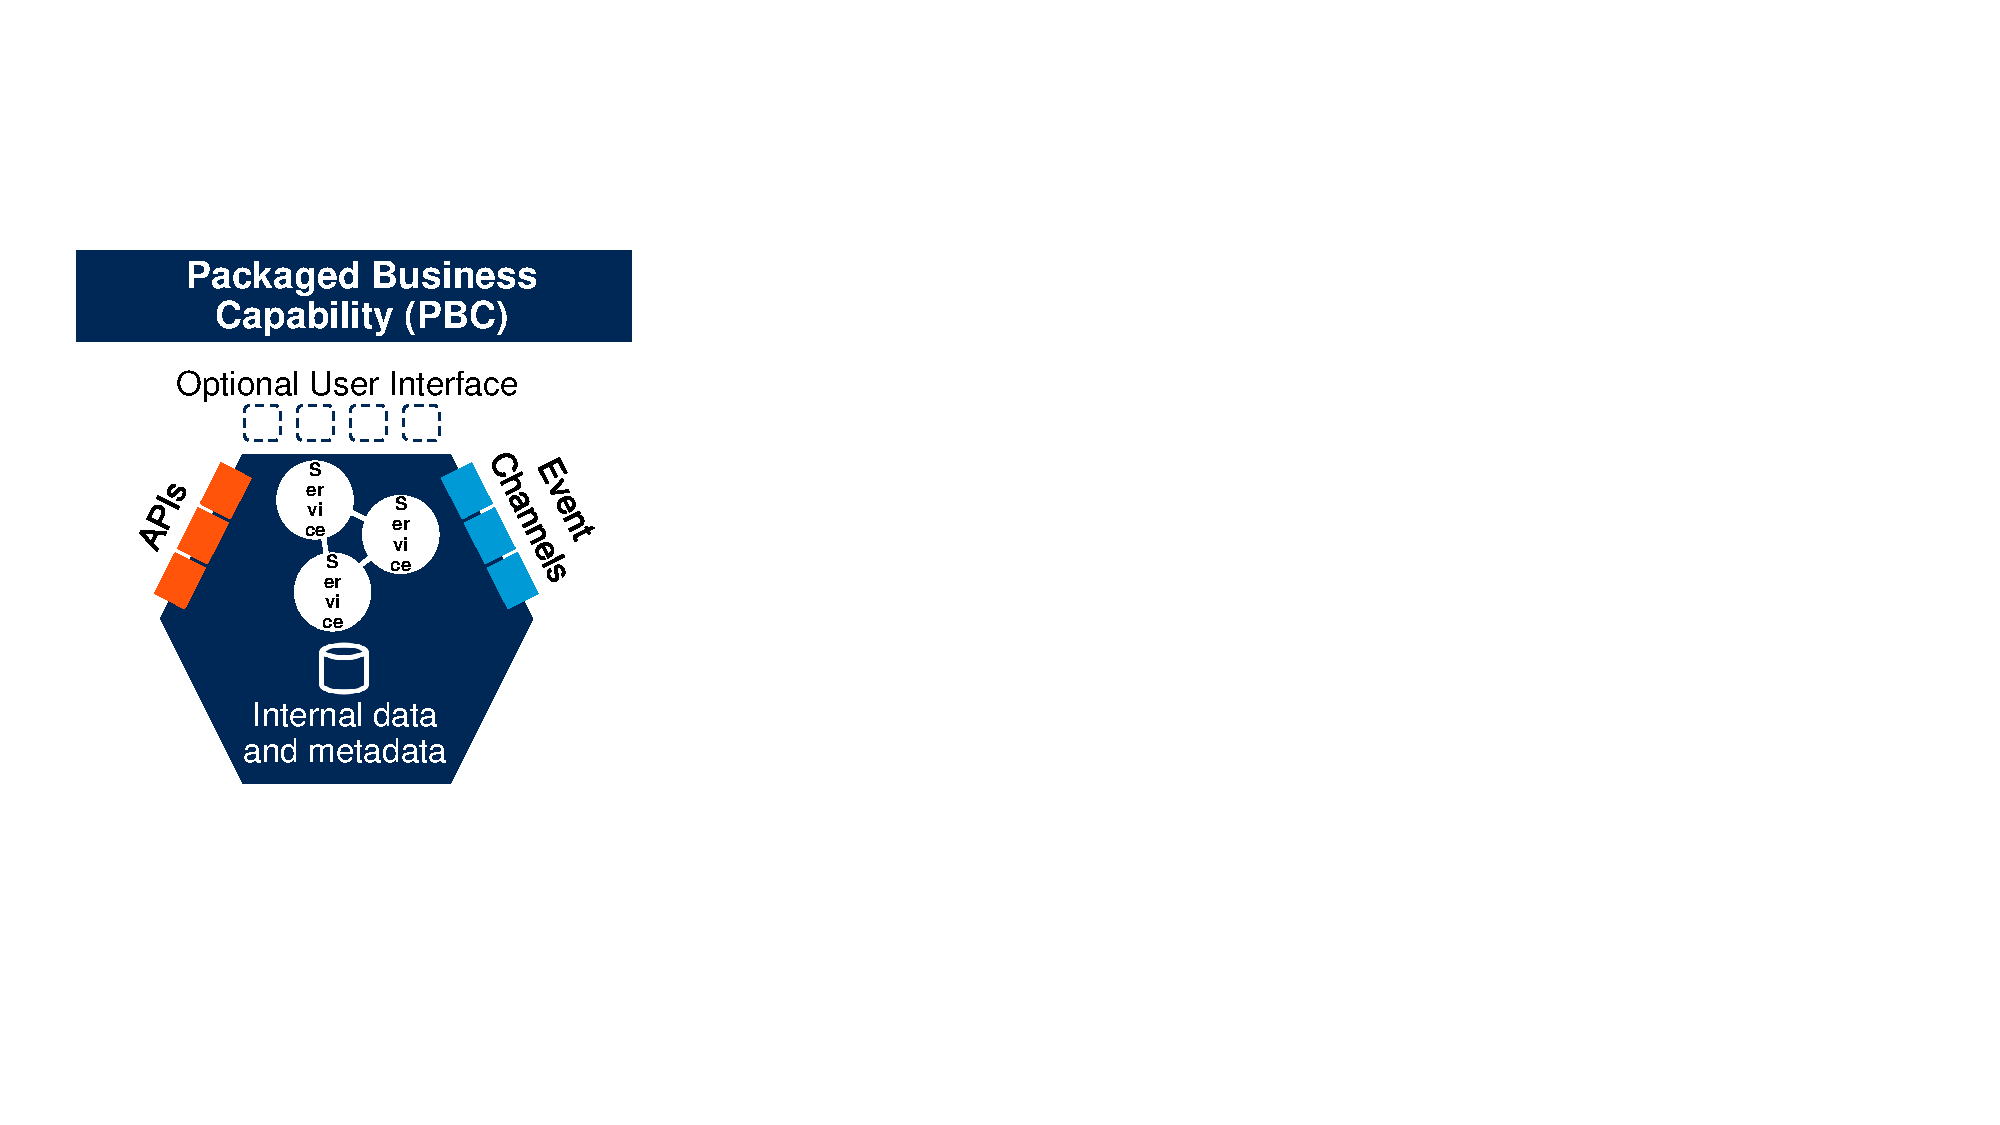
\includegraphics[scale=0.6]{figures/PBCstructure.pdf}
    \caption{Struttura \ac{PBC} secondo \textit{Gartner}}
    \label{fig:pbc-struttura}
\end{figure}

Questa struttura consente di progettare \textbf{applicazioni componibili}, assemblate combinando \ac{PBC} esistenti o sviluppandone di nuove.
Secondo \textit{Gartner}, tale approccio accelera il time-to-market, migliora l’adattabilità ai cambiamenti e garantisce soluzioni coerenti
con le esigenze operative dei clienti. Le applicazioni componibili sono progettate per richiamare dinamicamente i servizi dei
sistemi sottostanti, adottando un modello di integrazione process-centric, dove i processi di business guidano l’organizzazione
anziché i dati o le singole applicazioni. Questo tipo di applicazioni hanno una struttura che distingue chiaramente due livelli:

\begin{itemize}
    \item \textbf{frontend}, focalizzato sull’esperienza utente (UX) e costruito con interfacce intuitive,
    \item \textbf{backend}, dedicato alla logica applicativa, implementato tramite \ac{PBC} indipendenti.
\end{itemize}

Una delle caratteristiche distintive di \textit{Peer Network} è la capacità di trasferire su componenti di business, le \ac{PBC} appunto, le proprie
competenze di dominio e costruire con esse soluzioni componibili, invece di sviluppare software interamente personalizzati per ogni cliente.
Questo approccio è stato favorito dall’esperienza che l’azienda ha maturato in tanti anni di attività sulla piattaforma \ac{ERP} di
SAP\footnote{https://www.sap.com/italy/index.html}, che ha storicamente definito i principali standard internazionali nel settore.

Le soluzioni di \textit{Peer Network} semplificano il lavoro dei diversi attori di un processo di business, grazie a flussi operativi chiari e una
gestione meno complessa rispetto alle tradizionali piattaforme \ac{ERP}, come SAP. L'integrazione con la piattaforma \ac{ESI}, che funge anche da
repository per le \ac{PBC}, permette ai sistemi sviluppati di comunicare direttamente con gli \ac{ERP} aziendali. Questo processo non solo facilita
il recupero e l'elaborazione dei dati necessari, ma introduce anche una serie di funzionalità aggiuntive. Le informazioni così ottenute vengono
presentate attraverso interfacce grafiche progettate per ottimizzare usabilità ed efficienza operativa.

\section{Gestione Progetti}
Nel corso del tempo, nonostante gli sforzi per migliorare l’organizzazione e incrementare l’efficienza lavorativa, in \textit{Peer Network} sono
emerse difficoltà nel gestire contemporaneamente tutti i progetti. Questi ultimi si dividono in due principali categorie:

\begin{itemize}
    \item \textbf{progetti esterni}: soluzioni sviluppate per i clienti, denominate \ac{SBS},
    \item \textbf{progetti interni}, suddivisi ulteriormente in due tipologie:
        \begin{itemize}
            \item \textbf{ricerca e sviluppo}: attività principale è l'aggiornamento continuo delle \ac{PBC} per integrarle
            rapidamente nelle soluzioni destinate ai clienti e il conseguente miglioramento della piattaforma \ac{ESI};
            \item \textbf{software gestionale \ac{PAM}}: applicazione utilizzata internamente per il monitoraggio e la gestione del lavoro svolto dai dipendenti.
        \end{itemize}
\end{itemize}

Nel contesto di questa complessità operativa e dinamicità, i project manager e i dipendenti hanno individuato alcune problematiche generali.
La più evidente è la scarsità di personale rispetto al carico di lavoro, che porta gli sviluppatori a ricoprire più ruoli contemporaneamente,
sia all’interno dello stesso progetto sia su più progetti. Questo sovraccarico rende difficile per ciascuno svolgere al meglio i compiti assegnati.
Inoltre, i project manager, provenienti da un background tecnico, tendono ad adottare un approccio eccessivamente orientato agli aspetti tecnici,
trascurando l'analisi di dominio e la pianificazione strategica. Un ulteriore ostacolo è rappresentato dalla difficoltà nel delegare compiti: le
competenze sono concentrate in poche persone esperte e il coinvolgimento di risorse junior richiede tempo e sforzi per formazione e supervisione,
che spesso vengono percepiti come un rallentamento delle attività.

Per affrontare queste problematiche, l’azienda ha deciso di uniformare il più possibile la gestione dei progetti, adottando un approccio standardizzato
per l’intero ciclo di vita. Basandosi sui principi del \textbf{\ac{PMBOK}}\cite{project2021guide}, i project manager hanno quindi elaborato lo schema
del ciclo di vita ideale di un progetto in \textit{Peer Network}, riportato in \Cref{fig:fasi-progettuali}. Le future modifiche nella gestione dovranno
progressivamente allinearsi a questo modello.

Il ciclo di vita del progetto è stato suddiviso in tre fasi principali. La prima, denominata “Idea, Design, Economics”, prevede l’analisi iniziale di un
nuovo progetto, la progettazione, la definizione del budget e la stipula del contratto. La seconda fase “Progetto Software,” si concentra sull’analisi
approfondita dei requisiti, sulla pianificazione e sullo sviluppo, fino al rilascio del prodotto. La terza fase, “Supporto e Servizio,” riguarda l’assistenza
post-installazione e le attività di manutenzione correttiva per garantire il corretto funzionamento del sistema.

\begin{figure}
    \centering
    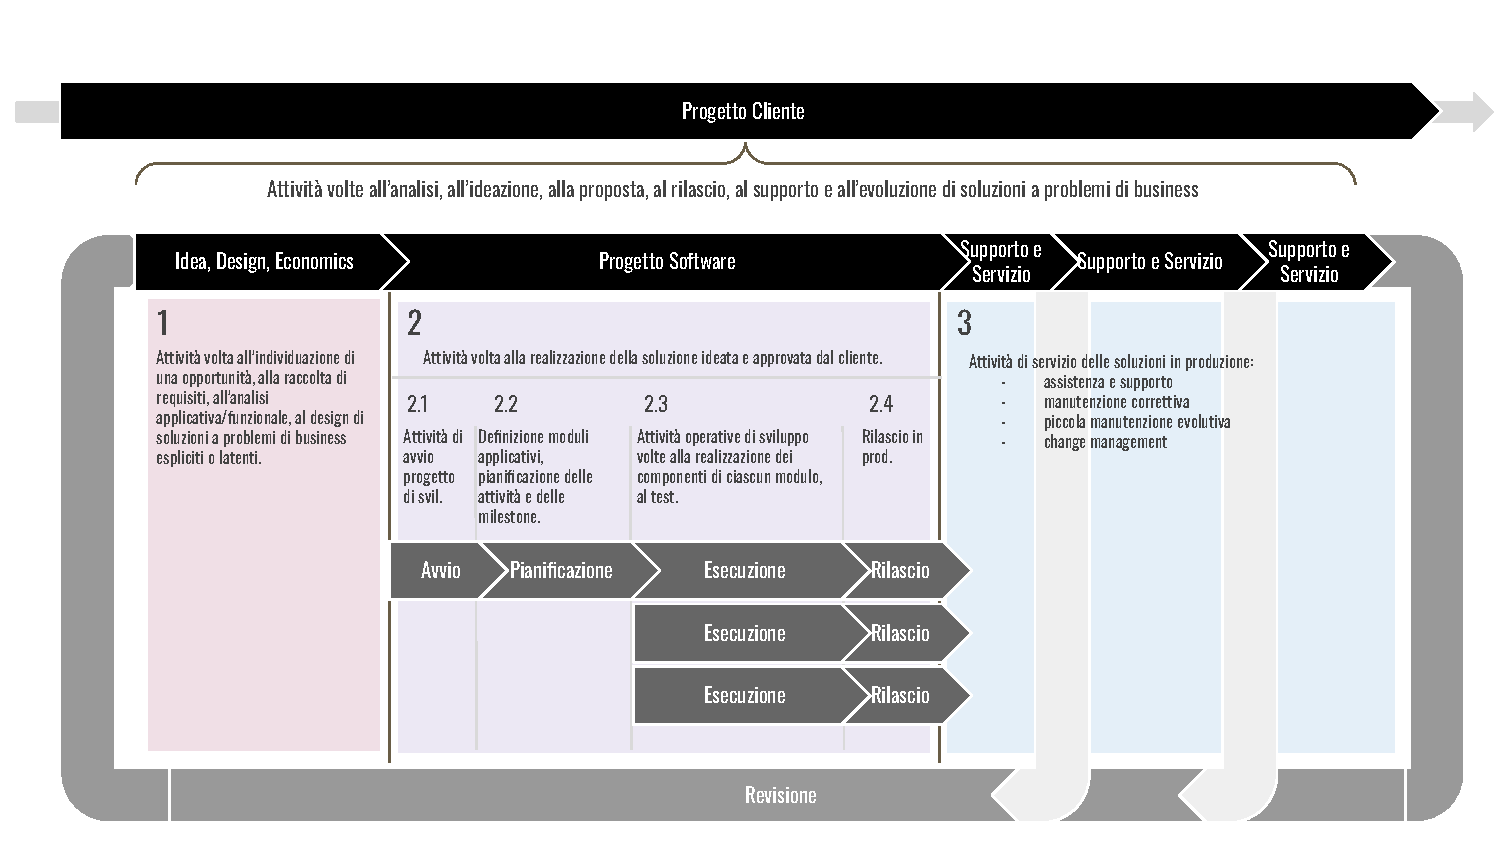
\includegraphics[width=\linewidth]{figures/FasiProgettualiPN.pdf}
    \caption{Ciclo di vita ideale per un progetto in \textit{Peer Network}}
    \label{fig:fasi-progettuali}
\end{figure}

Per raggiungere l'obiettivo di migliorare la gestione dei progetti, è innanzitutto fondamentale esaminare in dettaglio tutte le attività svolte nel novembre 2024,
identificando i problemi riscontrati dai dipendenti in ciascuna fase. Successivamente, basandosi sulle linee guida del \ac{PMBOK} e tenendo conto delle specifiche
esigenze aziendali, vengono proposti deliverables mirati, come schemi, analisi e documenti, per affrontare e risolvere le criticità emerse. Qualora alcune proposte
non risultassero applicabili per ragioni aziendali, vengono fornite spiegazioni che giustificano le decisioni adottate. Tutte queste informazioni vengono riportate
nel Capitolo \ref{chap:Contribution}.

\section{Peer Network Activity Management}
Il software interno \textbf{Peer Network Activity Management (PAM)} attualmente supporta l’amministrazione nella gestione delle risorse umane, nel monitoraggio e nella rendicontazione mensile
delle ore di lavoro dei dipendenti sui vari progetti, oltre a generare automaticamente report mensili da allegare alle fatture da inviare ai clienti.
Queste rappresentano le prime funzionalità implementate, considerate le più urgenti. Tuttavia, \ac{PAM} è stato concepito con una visione più ampia, mirata
alla gestione complessiva dell'azienda.

Per anni, il processo di fatturazione aziendale è stato gestito in modo poco strutturato e senza strumenti specifici, richiedendo circa due settimane
di lavoro mensile, oltre ad un contributo rilevante da parte dei project manager. Sebbene parzialmente automatizzato tramite il software Knime\footnote{https://www.knime.com},
il flusso di lavoro, illustrato in parte nella \Cref{fig:fatturazione-knime}, richiedeva una significativa supervisione manuale per avviare e monitorare ciascuna fase.
Inoltre, il processo prevedeva frequenti operazioni manuali di importazione ed esportazione di dati tramite diversi fogli elettronici Google
Sheet\footnote{https://workspace.google.com/intl/it/products/sheets/}.

\begin{figure}
    \centering
    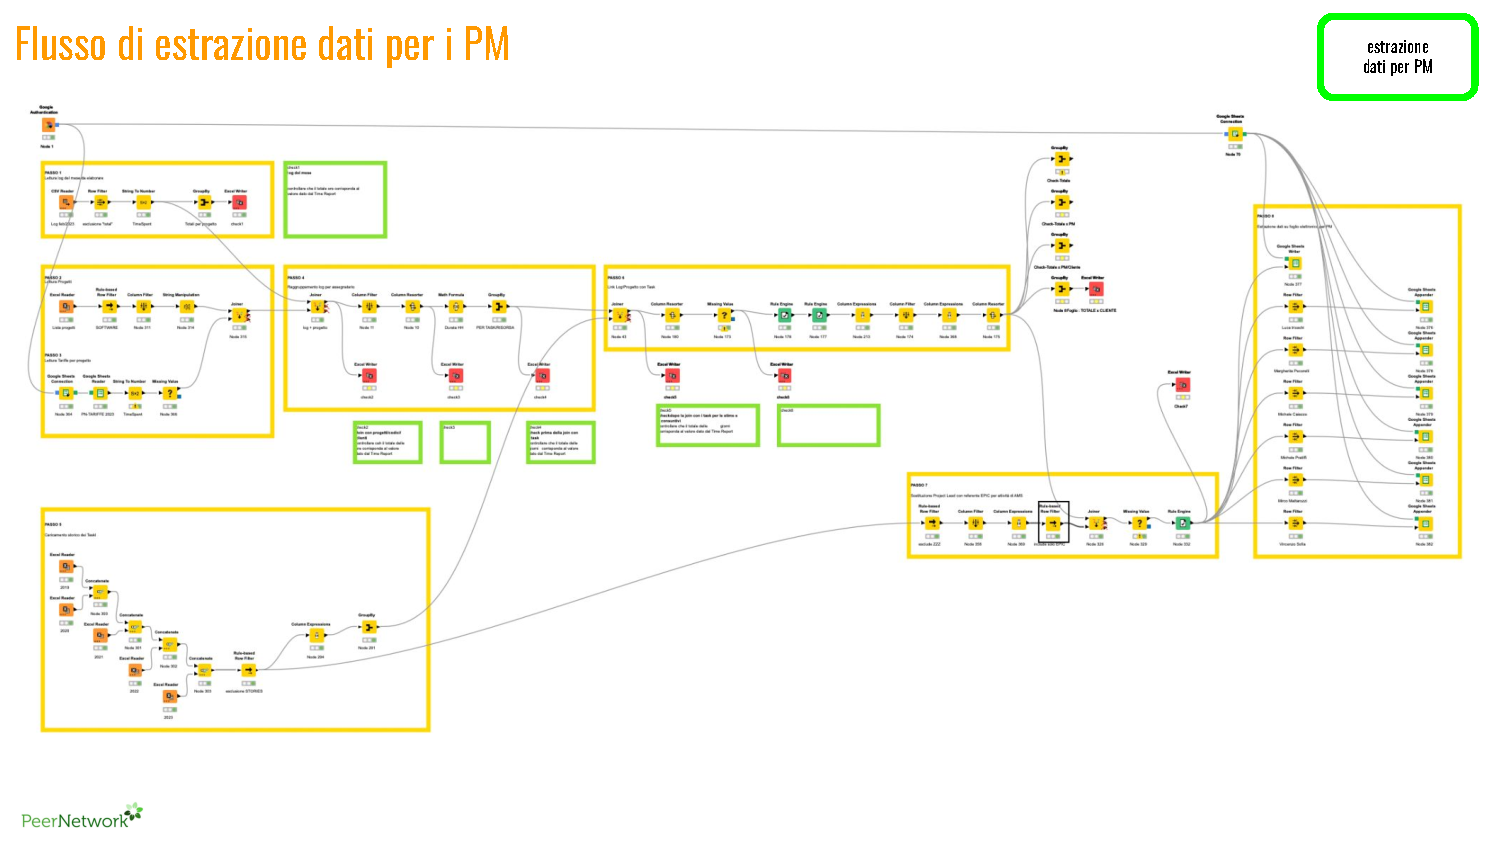
\includegraphics[width=\linewidth]{figures/FatturazioneKnime.pdf}
    \caption{Struttura su Knime riguardante una parte del processo di fatturazione, cioè l’estrazione di dati per i project manager}
    \label{fig:fatturazione-knime}
\end{figure}

Questo processo risultava troppo dispendioso in termini di tempo ed era basato su numerosi passaggi manuali. Per affrontare queste criticità, a gennaio 2024
è stato avviato il progetto interno \ac{PAM}, partendo con l’obiettivo di automatizzare gran parte del processo di fatturazione.
Le attività e il loro ordine di esecuzione sono schematizzate nella \Cref{fig:fatturazione}.

A partire da ottobre 2024, è stata resa disponibile la prima versione del sistema, che consente di completare l’intero flusso dal passaggio “estrazione dati
per PM” alla “generazione dei rapportini,” in poche ore anziché nelle circa due settimane precedentemente necessarie. L’utilizzo dei fogli elettronici da creare,
modificare o importare è stato completamente eliminato: l’intero processo è ora gestito dal gestionale, con l’utente che interagisce direttamente tramite un’unica
interfaccia grafica. L’automazione della fase di estrazione dati è stata resa possibile grazie all’integrazione con Jira\footnote{https://www.atlassian.com/software/jira},
uno strumento per la gestione e il monitoraggio dei progetti che consente ai dipendenti di registrare le ore lavorate su ciascun progetto.

\begin{figure}
    \centering
    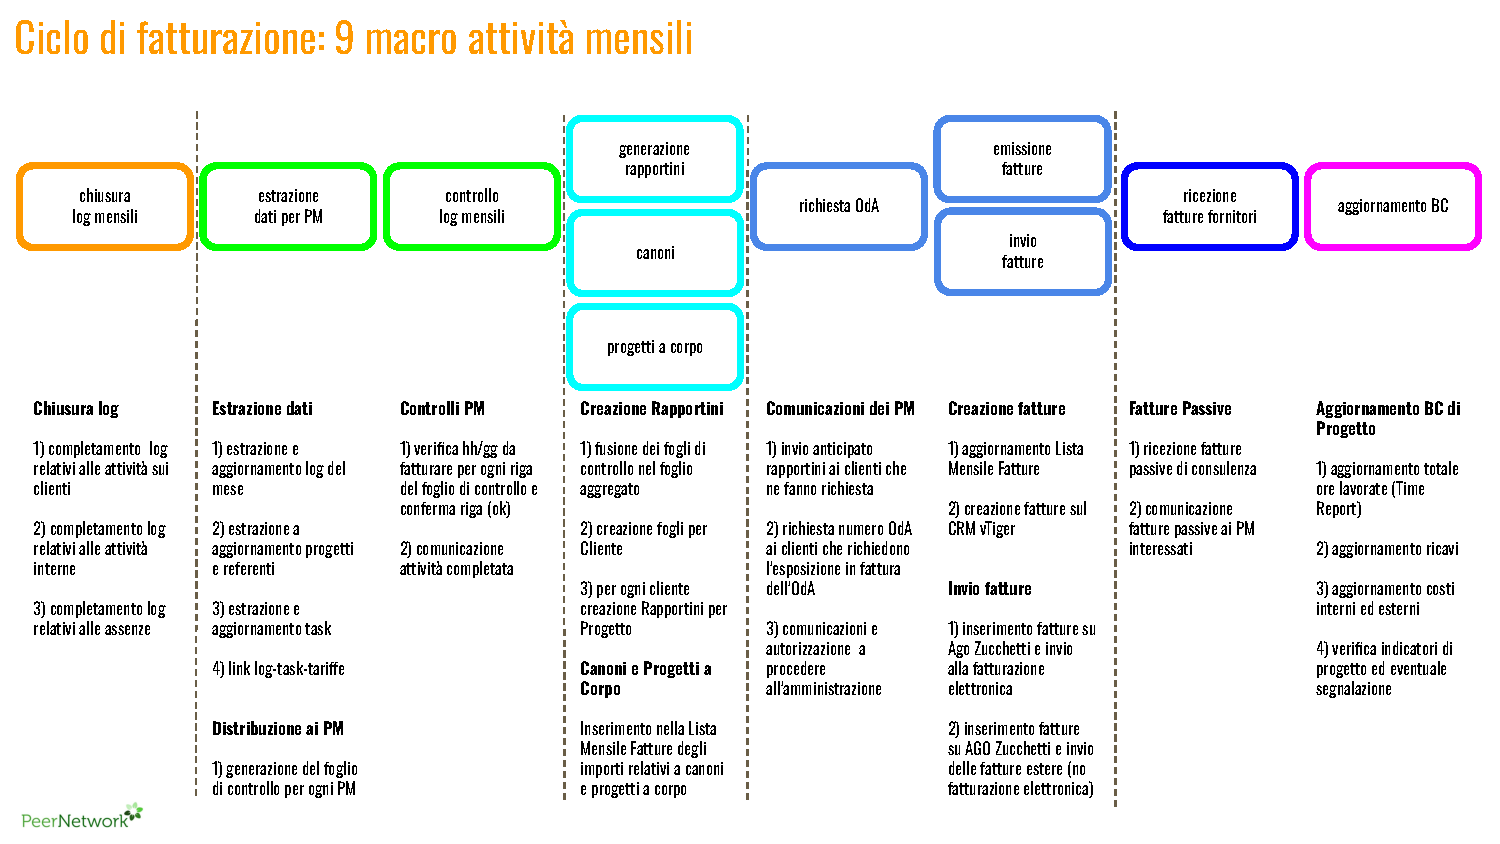
\includegraphics[width=\linewidth]{figures/fasiFatturazionePN.pdf}
    \caption{Attività presenti nel processo di fatturazione di \textit{Peer Network}}
    \label{fig:fatturazione}
\end{figure}

Le nuove funzionalità in fase di sviluppo, approfondite nel Capitolo \ref{chap:Results}, riguardano l’area dell’applicativo \ac{PAM} denominata \textbf{Progetti}, che verrà
utilizzata dalla direzione, dall’amministrazione e dai project manager. Questa sezione è pensata per centralizzare il controllo dei progetti, rendendo disponibili
informazioni generali, composizione dei team, tariffe orarie applicabili in base ai ruoli, situazione economica complessiva e dettagliata per mese, oltre alla
possibilità di consultare tutte le prefatture emesse.

Queste funzionalità semplificheranno notevolmente il lavoro degli utilizzatori, offrendo un unico punto di accesso per monitorare tutte le informazioni e mantenere
sotto controllo l’andamento dei progetti. Inoltre, la nuova gestione economica, sia generale che dettagliata, eliminerà la necessità di utilizzare i fogli elettronici
attualmente impiegati. Al momento, per ogni progetto viene creato un file separato per ogni anno solare, che deve essere aggiornato manualmente (come ultima fase del
processo di fatturazione nella \Cref{fig:fatturazione}) con i dati relativi a costi e ricavi effettivi, ricavi previsti per i mesi successivi e margini. Con la nuova area
Progetti, queste operazioni saranno automatizzate e integrate direttamente nell’applicativo.

\chapter{Strumenti e Tecnologie}
In questo capitolo vengono esaminati i principali strumenti e le tecnologie utilizzati durante lo svolgimento di tutte le attività, suddivisi in categorie
in base alla loro tipologia. Verranno trattati, con un approfondimento sul loro utilizzo pratico, gli ambienti di sviluppo integrati (IDE), i sistemi di
versionamento, i framework, le librerie e i linguaggi di programmazione, nonché le piattaforme per la gestione dei progetti e la collaborazione.
La scelta di queste tecnologie è stata influenzata principalmente dalle soluzioni già adottate da \textit{Peer Network} per la gestione e lo sviluppo dei progetti, 
oltre ad alcune proposte mirate a soddisfare esigenze operative specifiche.

\section{Strumenti}
\begin{itemize}
    \item \textbf{Jira}: strumento di gestione progetti e monitoraggio sviluppato da Atlassian, principalmente per i team di sviluppo software. Questo strumento
    supporta metodologie Agile e consente di creare, assegnare e monitorare le attività. Tutte le attività svolte sono state registrate, organizzate e monitorate
    in un apposito progetto. Ogni progetto è strutturato con una gerarchia di epic, task e subtask, permettendo di suddividere il lavoro in unità più piccole e
    gestibili, in modo da mantenere un controllo chiaro e dettagliato sui progressi. Gli elementi della gerarchia sono stati costantemente aggiornati con dettagli
    e stato corrente, garantendo una visione sempre aggiornata. Le ore di lavoro dedicate a ciascun task e subtask sono state registrate tramite una funzionalità
    specifica e monitorate facilmente con l’applicazione integrata \textbf{Time Tracker Lite}, utilizzando filtri per l’analisi dei dati. Per pianificare le varie attività
    da svolgere, è stata utilizzata la dashboard \textbf{Timeline}, che permette di avere una panoramica chiara delle scadenze e delle priorità. Jira è stato integrato con
    Confluence per collegare attività e documentazione dello stesso progetto.
    \item \textbf{Confluence}\footnote{\url{https://www.atlassian.com/software/confluence}}: strumento di collaborazione e gestione della conoscenza sviluppato da Atlassian, progettato per centralizzare la creazione, l'organizzazione
    e la condivisione di documenti e pagine. È stato utilizzato per documentare i progetti, raccogliere appunti e facilitare la collaborazione in tempo reale tra i colleghi.
    Integrato con Jira, ha permesso di collegare facilmente la documentazione alle attività monitorate, mantenendo coerenza tra sviluppo e gestione operativa. Ogni progetto
    è organizzato in uno spazio dedicato, dove sono raccolti resoconti di riunioni, documentazione tecnica e materiali di supporto, garantendo un accesso rapido e
    strutturato alle informazioni. La \textit{Peer Network} utilizza questo strumento per creare e mantenere una knowledge base aziendale, utile come riferimento per risolvere
    problemi ricorrenti e condividere best practice. Grazie alla sua flessibilità, Confluence ha reso possibile aggiornare costantemente i contenuti e organizzare le
    informazioni in modo chiaro e accessibile a tutti i dipendenti.
    \item \textbf{Bitbucket}\footnote{\url{https://bitbucket.org/}}: piattaforma di gestione del codice sorgente sviluppata da Atlassian, è stata utilizzata per tracciare e gestire in modo efficiente le
    modifiche al codice tramite il controllo di versione \textbf{Git}\footnote{\url{https://git-scm.com}}. L'azienda ha repository dedicati per ogni progetto, implementando rigorosi controlli di accesso che
    garantiscono sia la sicurezza che una gestione centralizzata del codice. Questa piattaforma aiuta la collaborazione tra i membri del team di sviluppo, consentendo
    a ciascun sviluppatore di contribuire al codice sorgente e monitorare in tempo reale le modifiche apportate dai colleghi.
    \item \textbf{Slack}\footnote{\url{https://slack.com/intl/it-it/}}: piattaforma di comunicazione e collaborazione aziendale progettata per ottimizzare il lavoro. Permette di inviare messaggi istantanei, effettuare
    chiamate vocali e video e condividere file in tempo reale. L’ambiente di lavoro \textit{Peer Network} è organizzato in canali tematici, suddivisi per progetto, reparto o argomento,
    facilitando la gestione delle conversazioni. Grazie all’integrazione con strumenti come Jira e Confluence, Slack supporta un flusso di lavoro collaborativo ed efficiente.
    Tutte le comunicazioni interne, sia tra colleghi che con l’azienda, sono state gestite tramite questa piattaforma, garantendo ordine e accessibilità alle informazioni.
    \item \textbf{Google Workspace}\footnote{\url{https://workspace.google.com/intl/it/}}: \textit{Peer Network} adotta un dominio aziendale dedicato tramite Google, fornendo a ciascun dipendente un account personalizzato
    per accedere agli strumenti e alle risorse condivise. Il \textbf{Google Drive} aziendale è stato utilizzato per archiviare, consultare e modificare file e cartelle, con permessi
    di accesso configurati per garantire sicurezza e controllo. I \textbf{Google Calendar} personali sono stati condivisi tra i dipendenti, facilitando la pianificazione di riunioni
    e attività. Le riunioni sono state programmate su Calendar e svolte in modalità mista, consentendo ai dipendenti in smart working di partecipare tramite \textbf{Google Meet}.
    Per le presentazioni, sono stati utilizzati \textbf{Google Slides}, sia per le riunioni interne che per quelle con i clienti. \textbf{Gmail} ha centralizzato tutte le notifiche aziendali,
    incluse quelle provenienti da strumenti come Jira, Confluence, Bitbucket e Slack, offrendo un unico punto di accesso per il monitoraggio delle comunicazioni e delle attività.
    \item \textbf{Miro}\footnote{\url{https://miro.com/it/}}: piattaforma di collaborazione online che ha semplificato la creazione e la condivisione in tempo reale di schemi e diagrammi, come la \textbf{\ac{WBS}},
    attraverso una lavagna virtuale accessibile a più colleghi simultaneamente. Miro è stato proposto all'azienda per sostituire l’uso di Google Slides, precedentemente impiegato
    per realizzare questi schemi senza uno strumento dedicato.
    \item \textbf{Visual Studio Code}\footnote{\url{https://code.visualstudio.com}}: editor di codice sorgente usato come IDE durante lo sviluppo. Grazie all'integrazione con Git e all'uso di alcuni plugin, ha consentito
    di gestire facilmente le operazioni di controllo versione direttamente dall’interfaccia grafica, semplificando il controllo del codice sorgente.
    \item \textbf{MySQL Workbench}\footnote{\url{https://www.mysql.com/products/workbench/}}: software dedicato alla gestione di database MySQL. Grazie alla sua interfaccia, è stato possibile consultare e interrogare il database di \ac{PAM}
    tramite la creazione e l’esecuzione di query SQL.
\end{itemize}

\section{Tecnologie}
\begin{itemize}
    \item \textbf{Vue.js}\footnote{\url{https://vuejs.org}}: framework JavaScript open-source progettato per la creazione di interfacce utente e applicazioni single-page. È noto per la sua reattività e
    facilità di integrazione con altre librerie. Basato su un’architettura a componenti, permette di organizzare il codice in moduli riutilizzabili e facilmente
    gestibili. Grazie ai suoi meccanismi reattivi, il \ac{DOM} si aggiorna automaticamente al variare dei dati, supportando direttive dinamiche
    per la manipolazione del contenuto. Questo strumento è stato impiegato per lo sviluppo frontend di \ac{PAM}.
    \item \textbf{Vuex}\footnote{\url{https://vuex.vuejs.org}}: libreria di gestione dello stato per Vue.js, progettata per centralizzare e organizzare i dati in un unico store. Facilita la gestione di
    applicazioni complesse grazie a un flusso strutturato di mutazioni, che consente di modificare lo stato in modo tracciabile e prevedibile. È particolarmente utile
    per condividere dati tra componenti senza la necessità di passaggi manuali. Questa libreria è stata utilizzata per lo sviluppo frontend di \ac{PAM}.
    \item \textbf{Liferay}\footnote{\url{https://www.liferay.com/it/}}: piattaforma open-source progettata per la creazione di portali web e siti aziendali, offrendo soluzioni personalizzate per la gestione di
    contenuti, applicazioni e servizi online. La sua architettura modulare garantisce elevata personalizzazione e scalabilità, rendendola adatta a progetti complessi.
    Supporta diversi framework e tecnologie, tra cui JavaScript, favorendo l’integrazione con strumenti moderni di sviluppo. Questa piattaforma è stata utilizzata per
    gestire il frontend di \ac{PAM}, ospitando il codice sviluppato in Vue.js.
    \item \textbf{JavaScript}\footnote{\url{https://developer.mozilla.org/en-US/docs/Web/JavaScript}}: linguaggio di programmazione utilizzato principalmente per lo sviluppo web. È eseguito direttamente nel browser e permette di creare
    pagine dinamiche e interattive. Viene utilizzato in Vue.js per creare e gestire i componenti e la logica dell'applicazione, oltre alla modifica dinamica del
    \ac{DOM} tramite direttive specifiche. Anche la gestione dello stato in Vuex è fatta in JavaScript.
    \item \textbf{MySQL}\footnote{\url{https://www.mysql.com/it/}}: sistema di gestione di database relazionali (RDBMS) utilizzato in \ac{PAM} per archiviare, organizzare e recuperare dati in modo strutturato.
    È stato possibile interagire con i dati tramite il linguaggio Structured Query Language (SQL). 
\end{itemize}

\chapter{Contribution}

You may also put some code snippet (which is NOT float by default), eg: \cref{lst:random-code}.

\lstinputlisting[float,language=Java,label={lst:random-code}]{listings/HelloWorld.java}

\section{Fancy formulas here}

\chapter{Results}
\label{chap:Results}

\chapter{Conclusion}

%----------------------------------------------------------------------------------------
% BIBLIOGRAPHY
%----------------------------------------------------------------------------------------

\backmatter

\nocite{*} % Remove this as soon as you have the first citation

\bibliographystyle{alpha}
\bibliography{bibliography}

%\begin{acknowledgements} % this is optional
%Optional. Max 1 page.
%\end{acknowledgements}

\end{document}
